\chapter{Założenia i~implementacja}
W poniższym rozdziale zaprezentowano założenia, potrzeby i~implementację systemu zbierania danych, opartego o~technologię LoRa.

\section{Założenia projektu}
System ma kilka podstawowych założeń:
\begin{itemize}
    \item jeden centralny punkt gromadzenia danych,
    \item zapisywanie danych do bazy danych szeregów czasowych w celu ich dalszego przetwarzania,
    \item zbieranie danych z dużego obszaru,
    \item niezależność od istniejących metod przesyłu danych (WiFi, sieci komórkowe, łączność satelitarna),
    \item niezależność od platformy sprzętowej,
    \item możliwie duża dostarczalność pakietów,
    \item dopuszczalne drobne opóźnienia w dostarczaniu danych.
          % \item węzły sieci tylko wysyłają dane, same nie konsumują przychodzących wiadomości.
\end{itemize}

\section{Części sieci}
W celu uzyskania wyżej wspomnianych założeń, zaproponowano system złożonych z~kilku części:
\begin{itemize}
    \item węzły sieci,
    \item stacje przekaźnikowe,
    \item broker wiadomości,
    \item baza danych.
\end{itemize}

Na rysunku~\ref{rys:system-diagram} przedstawiono schemat systemu.

\begin{figure}[p!]
    \begin{center}
        % 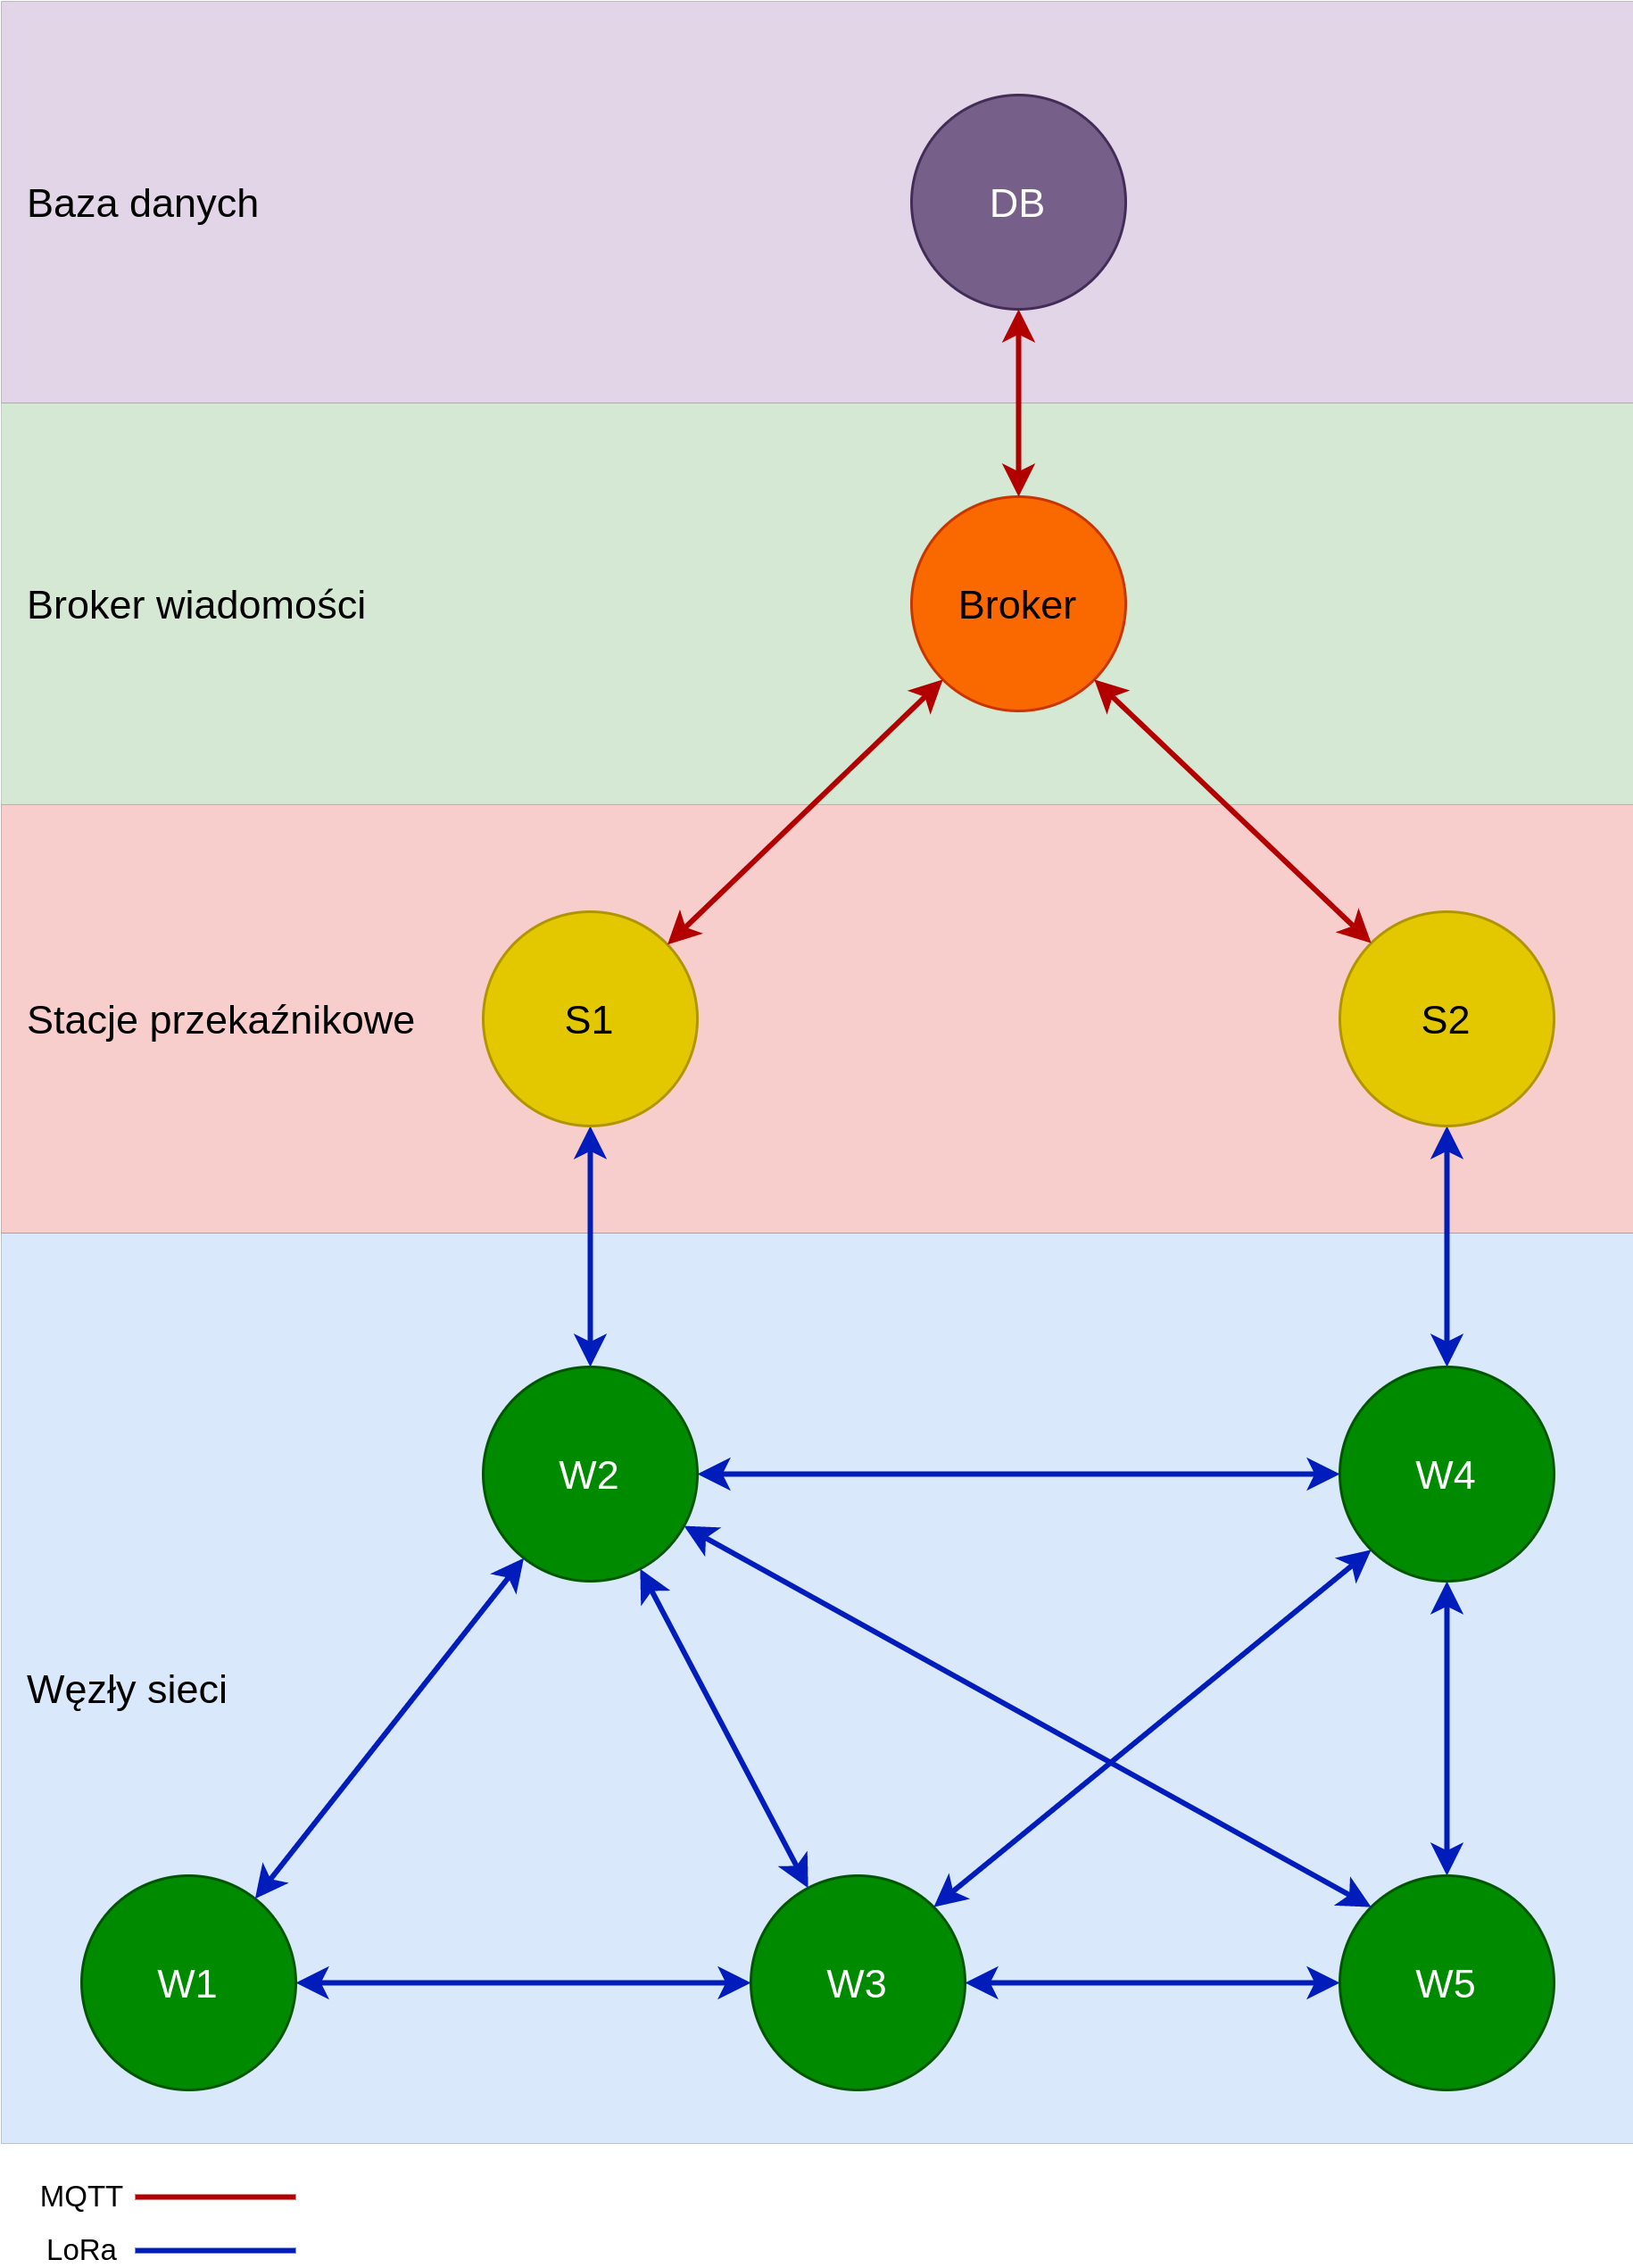
\includegraphics[width=3cm]{pic/diagram-systemu.png}
        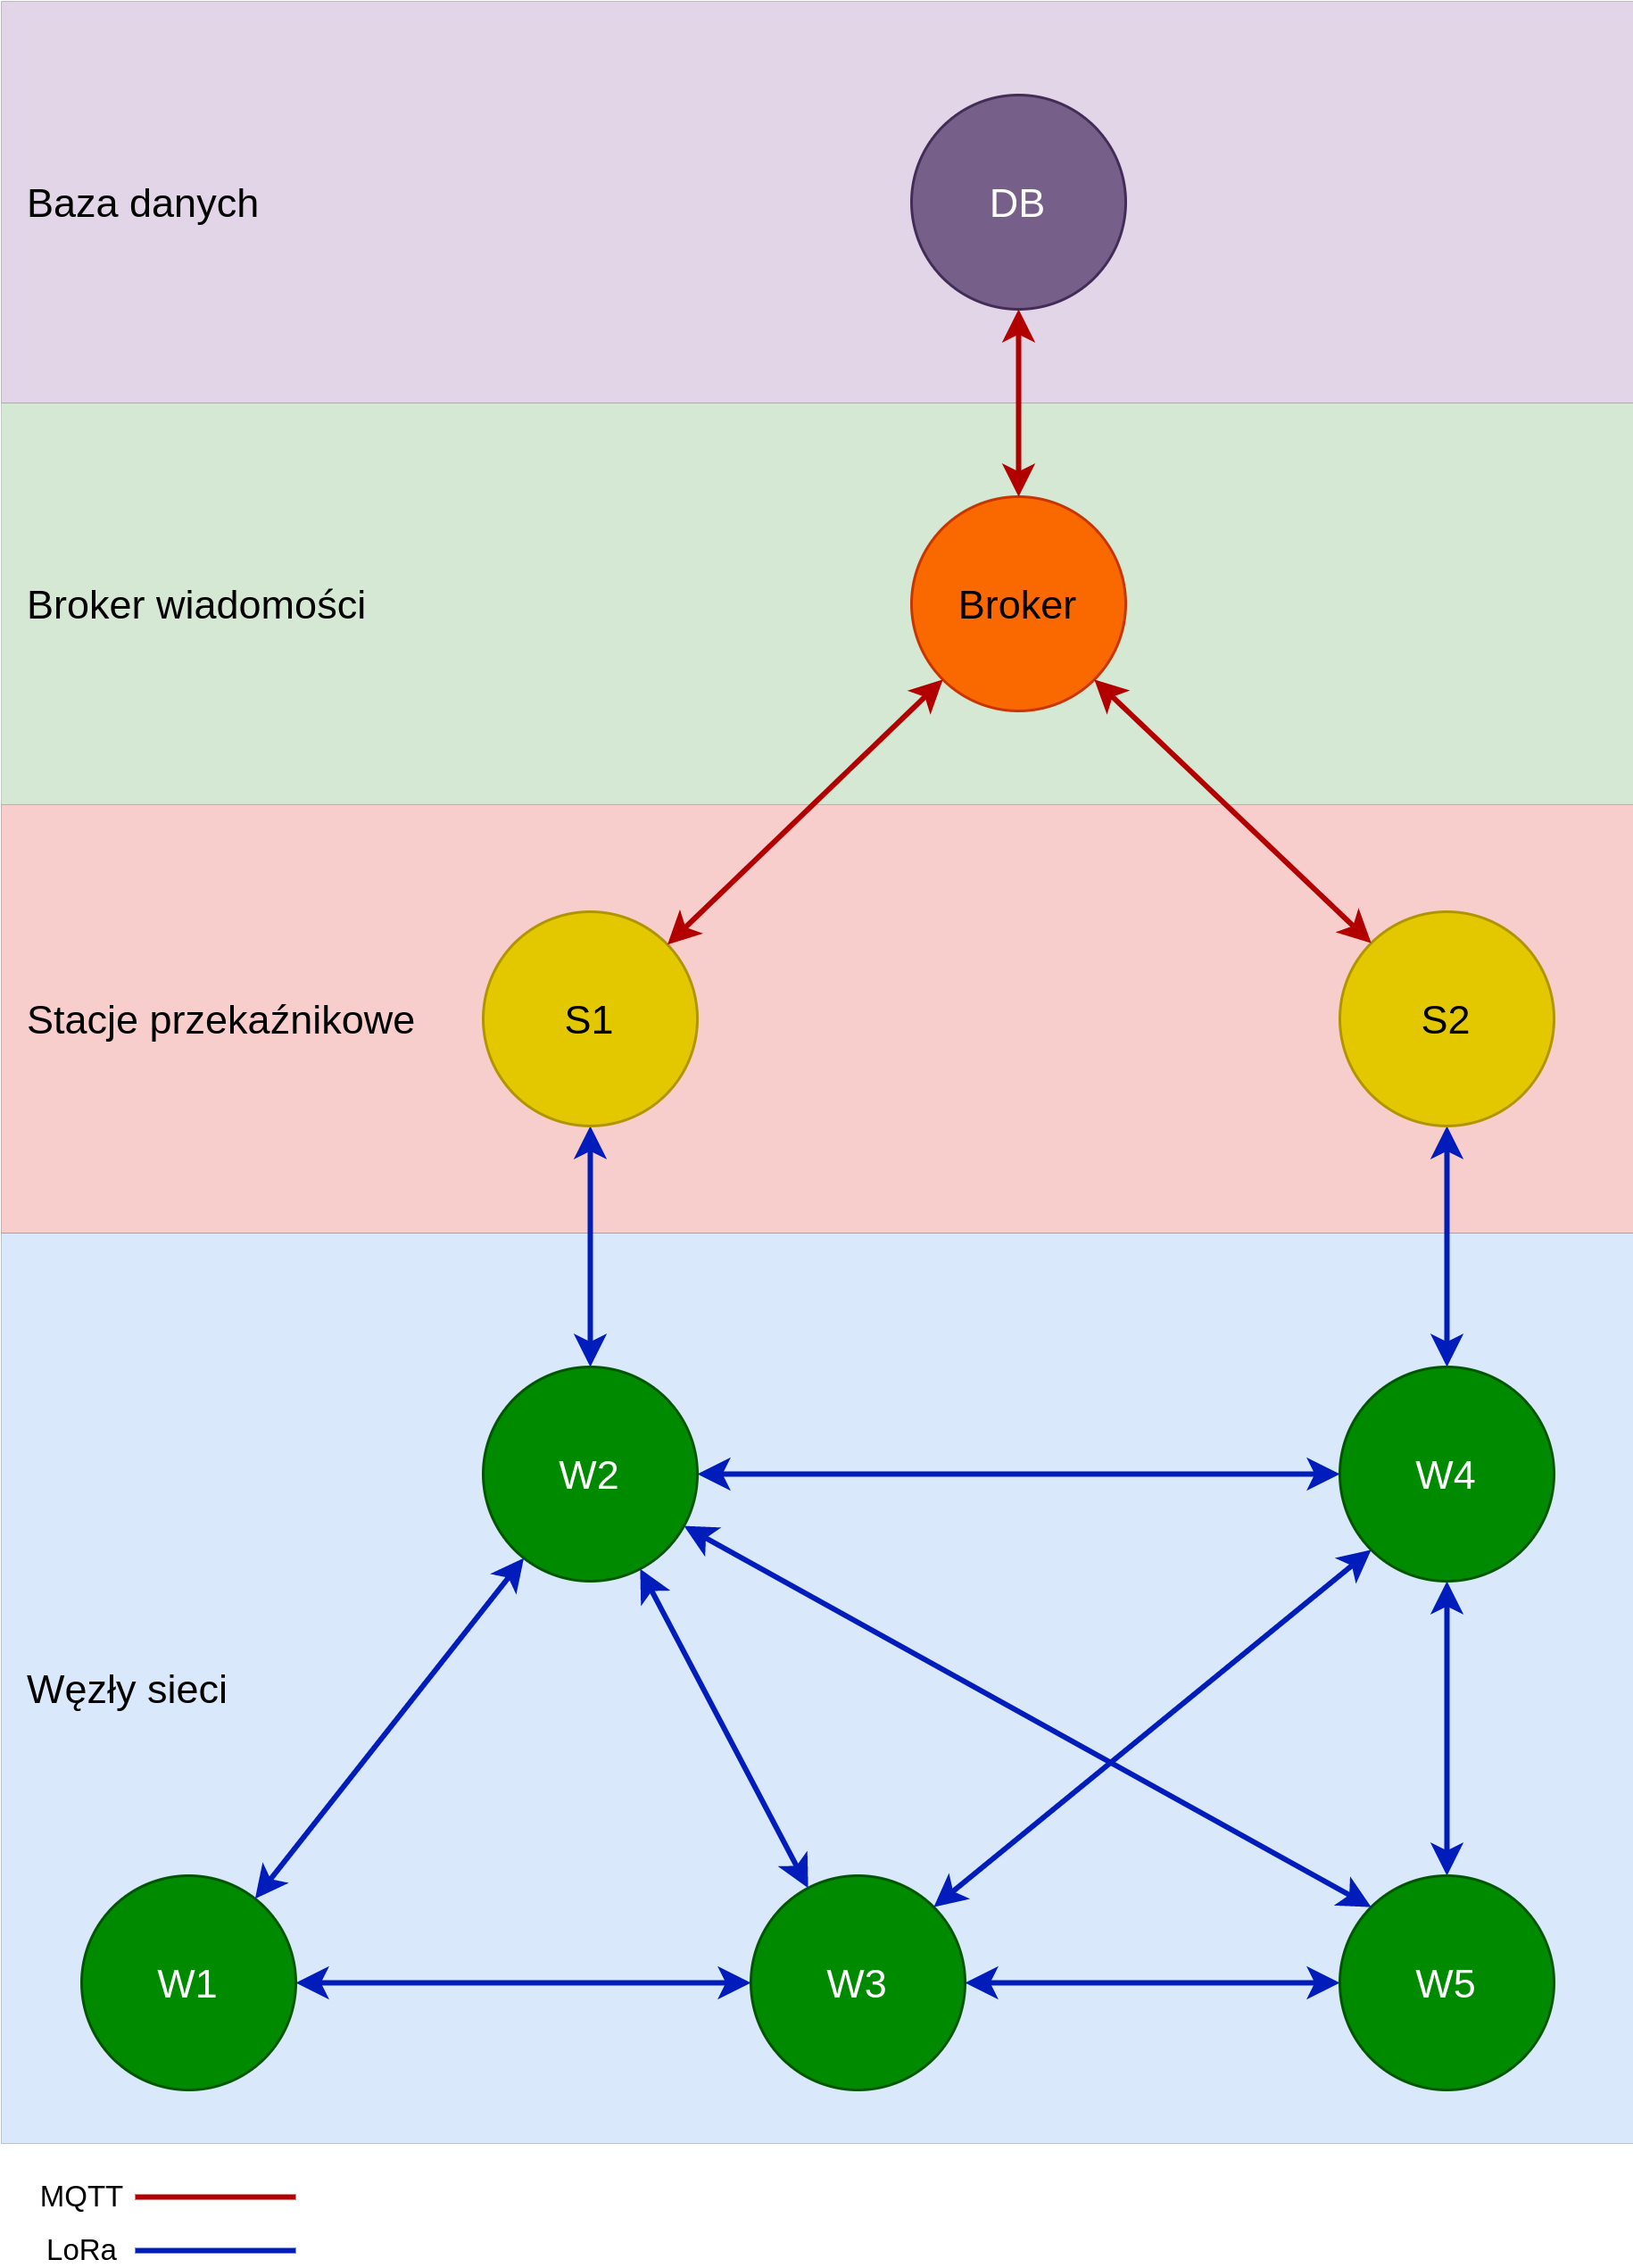
\includegraphics[width=15cm]{pic/diagram-systemu.png}
    \end{center}
    \caption{Diagram prezentujący schemat ideowy systemu}\label{rys:system-diagram}
\end{figure}

\subsubsection{Węzły sieci}
Węzły sieci to urządzenia wyposażone w moduł LoRa i~odpowiednie oprogramowanie pozwalające na pełną obsługę sieci.
Gdy węzeł odbierze wiadomość, sprawdza jej poprawność i~rozsyła ją dalej w celu zapewnienia jak największego zasięgu i~dostarczalności

Urządzenie to może być również wyposażone w~różnego rodzaju czujniki, które dostarczają danych do bazy danych.

\subsubsection{Stacja przekaźnikowa}
Stacja przekaźnikowa to urządzenie wyposażone zarówno w~moduł LoRa, jak i~moduł umożliwiający komunikację z~siecią Internet (np. moduł WiFI lub Ethernet).

Urządzenie to odbiera przychodzące wiadomości LoRa i~przesyła je do brokera wiadomości.

\subsubsection{Broker wiadomości}
Broker wiadomości to program, działający na komputerze mającym dostęp do sieci, umożliwia on wydajną komunikację pomiędzy stacją przekaźnikową a~bazą danych.

\subsubsection{Baza danych}
Baza danych umożliwia zapisywanie sporej ilości danych, uwzględniając również ich czas (baza danych szeregów czasowych).
O~zapis danych z brokera wiadomości do bazy danych dba osobny program, który powinien sprawdzać również poprawność tych wiadomości, jak i~dbać o~to by, nie zapisywać powtórzonych wiadomości.

\section{Wiadomości}
Każda z wiadomości przesyłanych za pomocą tych sieci powinna mieć format jak zaprezentowano na listingu~\ref{lst:packet_format}

Zawiera ona pola:
\begin{itemize}
    \item \texttt{ttl} — (ang. \emph{time to live} — czas życia) wartość określająca maksymalną liczbę skoków pomiędzy węzłami sieci. (domyślnie wynosi 10, może zostać wydłużona w~zależności od wielkości planowanej sieci);
    \item \texttt{m\_id} — UUID~\cite{RFC:uuid} wiadomości, gwarantujący niepowtarzalności tej wiadomości; ułatwia również jej dalsze przetwarzanie;
    \item \texttt{d\_id} — numer identyfikacyjny urządzenia, z~którego pochodzi wiadomość;
    \item \texttt{values} — słownik zawierający dane z~urządzenia, do zapisania w bazie.
\end{itemize}

\begin{lstfloat}[h!]
    % \begin{lstfloat}[b!]
    \lstset{language=JavaScript}
    % \lstset{}
    \begin{lstlisting}[frame=single]
{
    "ttl": 10,
    "d_id": "id_233",
    "m_id": "eaa17a7b-9388-43b6-9310-731c942fc6b9"
    "values": {
        "temp": 21,
        "hum": 50,
        "press": 1000,
        "light": 100,
        "co2": 1000,
        "pm25": 10,
        "pm10": 20
    },
}          
\end{lstlisting}
    \caption{Przykładowa wiadomość przesyłana przez system}\label{lst:packet_format}
\end{lstfloat}

\section{Obsługa protokołu}

\subsubsection{Działanie węzłów}
Wiadomości generowane są przez węzły sieci, zawierając wszystkie niezbędne pola (wymienione wyżej) i~odczyty z czujników zamieszczonych w~węźle.
Następnie zostaje ona rozesłana do wszystkich węzłów w~zasięgu (ang. \emph{broadcasting}).

Węzeł odbierając wiadomość, sprawdza jej poprawność (czy jest odpowiednio sformatowana, czy zawiera wszystkie potrzebne pola), i~jeżeli wiadomość jest poprawna, a~pole \texttt{ttl} jest większe od 0~rozsyła wiadomość dalej.
Sprawdzanie wiadomości odbywa się w~celu wyeliminowania wiadomości niepoprawnych z~sieci.

\subsubsection{Działanie stacji przekaźnikowej}
Stacja przekaźnikowa odbiera wiadomości i~przesyła je do brokera wiadomości.
Nie sprawdza poprawności wiadomości, by zapewnić maksymalną wydajność i~niezawodność.

\subsubsection{Działanie bazy danych i programu zapisującego dane}
Program pobiera kolejne wiadomości od brokera i~przetwarza je w~kolejności:
\begin{enumerate}
    \item sprawdzenie poprawności wiadomości;
    \item \label{itm:powtorki} upewnienie się, czy wiadomość nie została już sprawdzona (na podstawie pola \texttt{m\_id});
    \item zapisanie danych ze słownika \texttt{values} do bazy danych i~przyporządkowanie ich do \texttt{d\_id}, oznaczenie ich znacznikiem czasowym;
    \item zapisanie w pamięci \texttt{m\_id}, potem do wykorzystania w~kroku~\ref{itm:powtorki}.
\end{enumerate}
Baza danych powinna przechowywać dane, takie jak:
\begin{itemize}
    \item \texttt{d\_id} — identyfikator urządzenia,
    \item znacznik czasowy,
    \item wartość pomiaru,
    \item nazwa pomiaru.
\end{itemize}

\section{Implementacja}

\subsubsection{Implementacja węzłów sieci}
W wyniku pracy nad systemem zbierania danych przygotowano implementację węzłów sieci z~wykorzystaniem dwóch platform sprzętowych:
% TODO sprawdzić jakie dokładnie to modele
\begin{itemize}
    \item Raspberry Pi Pico,
    \item TTGO LoRa32.
\end{itemize}

\subsubsection{Raspberry Pi Pico}

W wyniku pracy nad systemem zostały przygotowane dwa identyczne urządzenia oparte o~Raspberry Pi Pico.
Urządzenie zostało wyposażone w moduł LoRa SX1262~\cite{PICO:sx1262-doc} (z wykorzystaniem płytki rozwojowej Waveshare SX1262 LoRa Node Module~\cite{PICO:waveshare-doc}) oraz czujnik temperatury i~wilgotności DHT11.
Urządzenie zostało zaprogramowane w~języku MicroPython z~wykorzystaniem biblioteki \texttt{micropySX126X}~\cite{PICO:lora-lib}.
Urządzenie wysyła wiadomości zawierające odczyty z czujnika co 5~minut.
Wysyłanie wiadomości odbywa się w~sposób asynchroniczny, dzięki czemu urządzenie może wykonywać inne operacje w tym czasie.

\subsubsection{TTGO T3 LoRa32}
W wyniku pracy nad systemem zostało przygotowane jedno urządzenie oparte o~TTGO LoRa32.
Urządzenie zostało wyposażone w~moduł LoRa SX1276~\cite{ESP32:sx1276-doc}.
Zostały one zaprogramowane w~języku C++ z użyciem PlatformIO — ekosystemu do programowania urządzeń IoT.~\cite{tool:pio}.
W programie zostały wykorzystane biblioteki:
\begin{itemize}
    \item \texttt{arduino-LoRa} — biblioteka do obsługi modułu LoRa~\cite{ESP32:lora-lib};
    \item \texttt{ArduinoJson} — biblioteka do obsługi formatu JSON~\cite{ESP32:ArduinoJson};
    \item \texttt{Adafruit-SSD1306} — biblioteka do obsługi wyświetlacza OLED~\cite{ESP32:Adafruit-SSD1306};
    \item \texttt{ESPRandom} — biblioteka do obsługi sprzętowego generatora liczb pseudolosowych~\cite{ESP32:ESPRandom}.
\end{itemize}
Urządzenie wysyła wiadomości zawierające odczyty z~czujnika co 5~minut.
Wiadomości zawierają wartości losowe, wygenerowane za pomocą sprzętowego generatora liczb pseudolosowych, zintegrowanego z~mikrokontrolerem ESP32.
Wysyłanie wiadomości odbywa się w~sposób asynchroniczny, dzięki czemu urządzenie może wykonywać inne operacje w~tym czasie.

\subsubsection{Implementacja stacji przekaźnikowej}
W wyniku pracy nad systemem zostało przygotowane jedno urządzenie oparte o~płytkę TTGO LoRa32.
Urządzenie zostało wyposażone w~moduł LoRa SX1276~\cite{ESP32:sx1276-doc} oraz moduł WiFi ESP32~\cite{ESP32:datasheet}.
Urządzenie zostało zaprogramowane w~języku C++ z~wykorzystaniem PlatformIO~\cite{tool:pio}.
W programie zostały wykorzystane biblioteki:
\begin{itemize}
    \item \texttt{arduino-LoRa} — biblioteka do obsługi modułu LoRa~\cite{ESP32:lora-lib};
    \item \texttt{Adafruit-SSD1306} — biblioteka do obsługi wyświetlacza OLED~\cite{ESP32:Adafruit-SSD1306};
    \item \texttt{WiFi} — biblioteka do obsługi modułu WiFi ESP32, zawarta w~pakiecie \texttt{arduino-esp32}~\cite{ESP32:Arduino};
    \item \texttt{PubSubClient} — biblioteka do obsługi protokołu MQTT~\cite{ESP32:PubSubClient}.
\end{itemize}

Urządzenie odbiera wiadomości LoRa i~przesyła je do brokera wiadomości za pomocą protokołu MQTT.
Wysyłanie wiadomości odbywa się w~sposób asynchroniczny, dzięki czemu urządzenie może wykonywać inne operacje w~tym czasie.
Urządzenie wyświetla na ekranie OLED informacje o~stanie sieci LoRa oraz otrzymanych wiadomościach.
Urządzenie nie sprawdza poprawności wiadomości, by zapewnić jak największą wydajność i~niezawodność.

\subsubsection{Implementacja brokera wiadomości}\label{impl:mosquitto}
Aby zapewnić niezawodność i~wysoką wydajność komunikacji zdecydowano użyć otwartoźródłowego brokera wiadomości Mosquitto~\cite{tool:mosquitto}.
Jest to sprawdzony, wydajny i~niezawodny program, który jest szeroko stosowany w systemach IoT, również w~zastosowaniach profesjonalnych~\cite{tool:mosquitto}.

\subsubsection{Baza danych}\label{impl:db}
W celu zapisywania danych zdecydowano użyć bazy danych InfluxDB 2.0~\cite{tool:influxdb}. Jest to baza danych szeregów czasowych, która jest wydajna i niezawodna~\cite{tool:influxdb}.

\subsubsection{Redis}\label{impl:redis}
W celu przechowywania identyfikatorów wiadomości, które zostały już sprawdzone, zdecydowano użyć bazy danych Redis.
Redis jest szybką, otwartoźródłową, nierelacyjną bazą danych typu \emph{klucz-wartość}, która jest jedną z~najczęściej stosowanych w~systemach informatycznych~\cite{tool:redis}.

\subsubsection{Program zapisujący dane}\label{impl:save}
W celu zapisywania danych zdecydowano użyć programu napisanego w~języku Python.
Program został napisany z~wykorzystaniem bibliotek:
\begin{itemize}
    \item \texttt{paho-mqtt} — biblioteka do obsługi protokołu MQTT~\cite{py:paho-mqtt};
    \item \texttt{influxdb-client} — biblioteka do obsługi bazy danych InfluxDB~\cite{py:influxdb};
    \item \texttt{redis-py} — biblioteka do obsługi bazy danych Redis~\cite{py:redis}.
\end{itemize}

Ostania wymieniona biblioteka została użyta do połączenia się z~bazą danych Redis, w~celu przechowywania identyfikatorów wiadomości, które zostały już sprawdzone.
Dzięki temu program nie zapisuje powtórzonych wiadomości do bazy danych.
